\documentclass[report.tex]{subfiles}

\begin{document}   

\section{Implementácia a grafické znázornenie}\label{sec:B}


\subsection{Prevedenie úlohy LP do tvaru pre \pyth|scipy.optimize.linprog|}

Metóda \pyth|linprog| z modulu \pyth|scipy.optimize| vyžaduje nasledujúci tvar úlohy LP:

\begin{align*}
	\text{min}~ &c^Tx\\
	&A_{ub}x \leq b_{ub} \\
	&A_{eq}x = b_{eq} \\
	&x \in [l, u] & l \leq u;~l,u \in (\mathbb{R}\cup \{-\infty, \infty\})^n 
\end{align*}

Hodnotami $-\infty$ a $\infty$ značíme neohraničenosť v danom smere, v zdrojovom kóde sa obe nahrádzajú hodnotou \pyth|None|. Upravme teda úlohy vyjadrené vyššie do predpísaného tvaru.

Pre $L^1$ lineárnu regresiu:

\begin{align*}
	\text{min}~ &
	\left(
	\begin{array}{c|c}
		\mathbf{0}_{k+1}^T & \mathbf{1}_n^T
	\end{array}
	\right)
	\left(
	\begin{array}{c}
		\beta \\
		\hline
		t
	\end{array}
	\right) \\
	&\left(
	\begin{array}{c|c}
		-\mathbf{A} & -\mathbb{I}_n \\
		\hline
		\mathbf{A} & -\mathbb{I}_n
	\end{array}
	\right)
	\left(
	\begin{array}{c}
		\beta \\
		\hline
		t
	\end{array}
	\right)
	\leq
	\left(
	\begin{array}{c}
		-y \\
		\hline
		y
	\end{array}
	\right) \\
	&\beta_i \in (-\infty, \infty) &i = 0,1,\dots,k\\
	&t_j \in [0, \infty) &j = 1,\dots,n
\end{align*}

Pre $L^{\infty}$ regresiu:

\begin{align*}
	\text{min}~ &
	\left(
	\begin{array}{c|c}
		\mathbf{0}_{k+1}^T & 1
	\end{array}
	\right)
	\left(
	\begin{array}{c}
		\beta \\
		\hline
		\gamma
	\end{array}
	\right) \\
	&\left(
	\begin{array}{c|c}
		-\mathbf{A} & -\mathbf{1}_n \\
		\hline
		\mathbf{A} & -\mathbf{1}_n
	\end{array}
	\right)
	\left(
	\begin{array}{c}
		\beta \\
		\hline
		\gamma
	\end{array}
	\right)
	\leq
	\left(
	\begin{array}{c}
		-y \\
		\hline
		y
	\end{array}
	\right) \\
	&\beta_i \in (-\infty, \infty) &i = 0,1,\dots,k\\
	&\gamma \in [0, \infty)
\end{align*}

Úlohy v zdrojovom kóde sú implementované práve v tomto tvare.

\subsection{Implementovanie regresných LP úloh}

Na implementáciu formulovaných LP úloh využívame tri knižnice:

\begin{itemize}
	\item \pyth|numpy| - tvorenie matíc a vektorov, načítanie dát
	\item \pyth|scipy.optimize| - implementovaný LP solver
	\item \pyth|matplotlib.pyplot| na vykresľovanie grafov.
\end{itemize}

Dáta relevantné pre túto úlohu sú uložené v súbore \verb|data/A04plotregres.npz|. Jedná sa o 16 bodov v $\mathbb{R}^2$, kde prvá súradnica reprezentuje nezávislú premennú (vektor týchto súradníc označíme \pyth|x|) a druhá závislú premennú (označíme \pyth|y|). 

\newpage

Vytvorme si potrebné štruktúry pre využitie metódy \pyth|scipy.optimize.linprog| pre LP formuláciu s $L^1$ normou:

\begin{python}
c = np.array([0,0] + [1] * len(x)) #objective function vector, two zeros stand for betas
A = np.matrix([[1] * len(x), x]).transpose()  
I = np.identity(len(x)) # Identity matrix

A_ub = np.block([[-A,-I], [A,-I]]) #creating a block matrix 
b_ub = np.concatenate([-y, y]) #right side vector
bounds = [(None, None), (None, None)] + [(0, None) for _ in range(len(x))] # bounds for variables
\end{python}

Pomocou solvera získame vektor optimálnych $\beta$ koeficientov:

\begin{equation*}
	\beta_0^{(1)} \approx -9.8378,~\beta_1^{(1)} \approx 2.1297
\end{equation*}

Podobne implementujeme $L^{\infty}$ formuláciu:

\begin{python}
c_inf = np.array([0,0,1]) #objective function vector
A_inf = np.matrix([[1] * len(x), x]).transpose() 
i_inf = np.array([[1] * len(x)]).transpose() # vector of ones

A_ub_inf = np.block([[-A_inf, -i_inf], [A_inf, -i_inf]]) # creating a block matrix
b_ub_inf = np.concatenate([-y, y])#right side vector
bounds = [(None, None), (None, None), (0, None)]
\end{python}

Znovu, pomocou solvera získame vektor optimálnych $\beta$ koeficientov:

\begin{equation*}
	\beta_0^{(\infty)} \approx 15.4545,~\beta_1^{(\infty)} \approx 1.7045
\end{equation*}

Pomocou získaných $\beta$ koeficientov vykreslíme regresné priamky spolu s pôvodnými dátami.

\begin{figure}[h!]
	\centering
	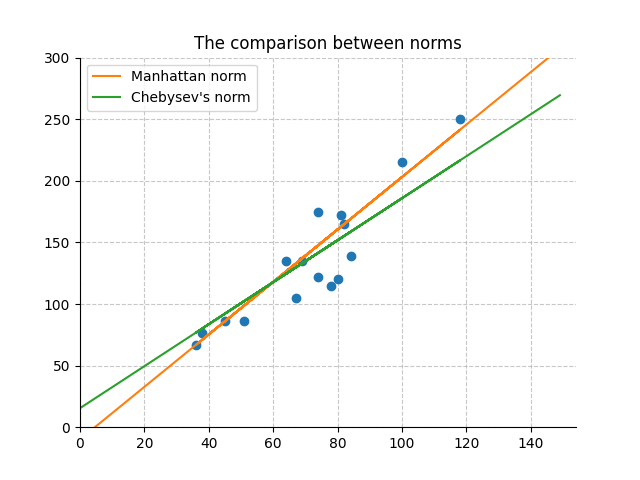
\includegraphics[scale=0.65]{figs/task_b_plot.png}
\end{figure}

\end{document}
